\section*{Introduction}
The EASIER detectors  goal is to measure the emission  from EAS in the
radio frequencies.  Each EASIER detector  is integrated in an Auger SD
and is composed  of antenna and an amplifier,  a power detection level
to transform  the HF  signal into its  power level, and  an adaptation
board    to    fit    the    Auger    SD    acquistion    front    end
(cf.~\ref{fig:detscheme}).\\  We   review  here  the   method  of  the
detector's  simulation in  the  C-band.  In  order  to understand  our
detector and  verify that our  simulation reproduce the data,  we will
often look at  the ratio of the noise fluctuation  over its mean. This
parameter  allows   us  to  probe  the  simulation   of  the  detector
independently  of  parameters  like  the  system  temperature  or  the
absolute  gain.  \\We will  first  look  at  the power  detection  and
adaptation board simulation.   Then we will step back  in the chain to
focus  on  the  HF  waveform  simulation from  a  frequency  spectrum.
Finally we will compare the simulation with the data.
\begin{figure}[!ht]
  \centering
  \hspace*{-3ex}
  \subfigure{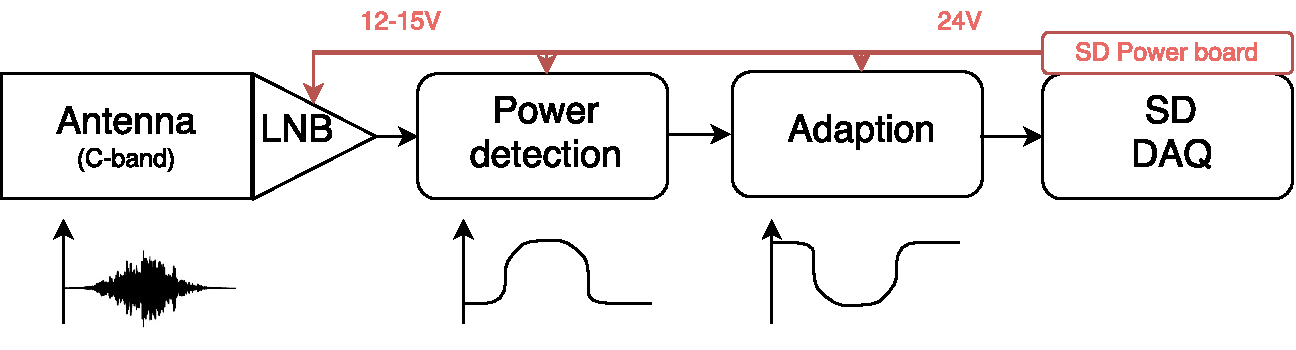
\includegraphics[width=0.60\linewidth]{blockdiagram.pdf}}
  \caption{}
  \label{fig:detscheme}
\end{figure}
\subsection*{EASIER detectorS}
Before going  into the  detail of the  simulation, we remind  the main
differences  between  the three  setups  that  were  installed in  the
C-band.   Three  different  detector  type were  installed,  the  main
difference is the antenna, but there  is also the presence or not of a
capacitor after  the power detector  that was removed after  the first
setup. The  table \ref{tab:easierdetectors} shows  the main difference
between those setups.

\begin{table}[h!]                                                                    
  \centering                                                                         
  \caption{bandwidths}                                                               
  \label{tab:easierdetectors}  
  \begin{tabular}{|c||c|c|c|}                                                        
    \hline                                                                           
    & EASIER 7 (setup 1)  & EASIER61 (setup 2) & GIGADUCK (setup 3) \\                                          
    \hline                                                                           
    antenna type & GI301  & DMX & Norsat \\                                          
    \hline                                                                           
    capacitor & yes  & no & no \\     
    \hline                                                                           
  \end{tabular}                                                                      
\end{table} 


%% The detector is integrated into  an Auger surface detector, i.e. it is
%% physically attached to  it and makes use of  the tank's trigger, power
%% supply  and acquisition.  Several  bands were  explored, the  VHF band
%% (30-80MHz), the  L-band (1-1.4 GHz)  and the C-band (3.4-4.2  GHz). We
%% focus here only on the C-band. 
%%  In this frequency band, three types of
%% detector  were  installed they  can  be  distinguished  mainly by  the
%% antenna used: the first array is composed of seven antennas We review
%% here the simulation  method for EASIER signal from  the radio spectrum
%% to the ADC trace.  Studies were already done on that subject, but push
%% here a  little further the  s A similar  study was already done  in my
%% thesis.  We  have implemented new  method of simulation for  the power
%% detector  and a more  precise way  to simulate  the EASIER  board.  We
%% looked  at  other  methods  for  the  power  detector  simulation  and
%% implemented a  more precise  way to simulate  the EASIER  board. \\The
%% motivation for this  study was to reproduce the RMS  of the data trace
%% with simulation in ADC. This is presented The new step is presented in
%% the second  section where  the data and  the simulation  are compared.
%% For this purpose  we use the RMS  of the radio signal in  ADC.  In the
%% last part we study the meaning  of the sigma mu ratio, i.e.  the ratio
%% of the noise fluctuation and the baseline value.
